\fancypagestyle{plain}{%
    \fancyhf{}
    \fancyhead[RO,LE]{\bfseries \thepage}
    \fancyhead[CO]{\rightmark}
    \fancyhead[CE]{\leftmark}
    \renewcommand{\headrulewidth}{0.4pt}}

\chapter{Lorentzova i Poincar\'{e}ova simetrija}

Iz dosadašnjih poglavlja trebalo bi biti jasno da je moć
neke simetrije to veća što je odgovarajuća grupa veća, što
će za kontinuirane (Liejeve) grupe obično značiti da je broj generatora
grupe veći. Stanja fizikalnih sustava i jednadžbe ili lagranžijani
koji tim sustavima upravljaju
će u tom slučaju biti više ograničeni zahtjevima kovarijantnosti
na transformacije simetrije i predviđanja koja su posljedica
primjene teorije grupa će biti netrivijalnija i općenitija.
Dodatnu moć simetrije dobivaju od netrivijalnih komutacijskih
relacija između generatora simetrija.
Tako već i razmjerno jednostavana simetrija na rotacije ima izuzetno
netrivijalne posljedice, kako smo vidjeli u poglavlju \ref{ch:rotacije}.
Prirodno je onda postaviti pitanje koja je maksimalna
simetrija koju teorije prirode moraju poštivati. Osim rotacija,
maksimalna grupa simetrija svakako treba sadržavati i translacije
u prostoru i vremenu, koje smo sreli u odjeljcima
\ref{sec:prostornetranslacije} i \ref{sec:vremensketranslacije}.
Već i kombiniranje ovih transformacija u istu grupu simetrija
nije trivijalno jer translacije i rotacije ne komutiraju. To je
vidljivo i iz običnih razmatranja geometrije u prostoru, a i iz 
neiščezavajućih komutacijskih relacija odgovarajućih
kvantnomehaničkih operatora impulsa $\vec{p}$ i momenta
impulsa $\vec{J}$.

\begin{equation}
    [J_{i}, p_{j}] = \rmi \hbar \epsilon_{ijk} p_{k} \;.
    \label{eq:jpkomutacijske}
\end{equation}

Pokazuje se da osim upravo navedenih transformacija, maksimalna
grupa simetrija koja upravlja najuniverzalnijim poznatim zakonima
prirode, onima kvantne teorije polja, od kontinuiranih prostornovremenskih
transformacija sadrži još samo Lorentzove transformacije među inercijalnim sustavima,
poznate kao Lorentzovi \emph{potisci} (engl. \emph{boost}).
Ta maksimalna grupa se obično naziva Poincar\'{e}ova\footnote{Priroda poštuje
    i općenitije trasformacije prostorvremena poznate kao difeomorfizmi. 
    Odgovarajuće simetrije poštuje klasična Einsteinova teorija gravitacije, ali još
    ih nismo uspjeli ugraditi u univerzalne kvantne teorije ostalih sila i
    tim simetrijama se ne bavimo u ovoj knjizi. Ne bavimo se ni \emph{konformnom}
    grupom simetrija koja Poincar\'{e}ovim transformacijama dodaje i
    dilatacije $x^{\mu}\to\lambda x^{\mu}$ što je simetrija koja prema
    trenutnim spoznajama nije egzaktna simetrija prirode,
    ali je svejedno od velikog teorijskog interesa.}.
Prije nego se pozabavimo Poincar\'{e}ovom grupom i njenim reprezentacijama,
pogledat ćemo prvo u sljedeća dva odjeljka grupno-teorijska svojstva samih
Lorentzovih potisaka koji, kako ćemo vidjeti, ne tvore grupu samostalno
nego tek u kombinaciji s rotacijama.


\section{Lorentzova grupa}
\label{sec:lorentz}

Einsteinova specijalna teorija relativnosti počiva na tzv.
principu relativnosti. Prema njemu, postoji skup ekvivalentnih koordinatnih
sustava (zvanih \emph{inercijalni sustavi})
u međusobnom jednolikom pravocrtnom gibanju, a u kojima fizikalni zakoni i pojave
izgledaju isto. Promatrač ne može eksperimentalno detektirati da 
se giba, ako se giba jednoliko. Mirovanje nije apsolutno,
čega su na ovaj ili onaj način bili svjesni već Kopernik, Galilei i Newton, ali je
tek Einstein uočio druge radikalne posljedice ovog načela, poput toga
da ni simultanost događaja nije apsolutna.
Princip relativnosti je princip simetrije na troparametarski skup transformacija
koje preslikavaju inercijalne sustave jedan u drugi.
Da bismo vidjeli o kojoj se grupi simetrija radi (i da li se uopće radi o grupi),
moramo ustanoviti kako se kombiniraju transformacije među inercijalnim sustavima.

Kako je poznato, iz principa relativnosti slijedi da
transformacije iz sustava $S=\{t,x,y,x\}$ u sustav $S'=\{t',x',y',x'\}$, 
tzv. \emph{Lorentzovi potisci}, imaju oblik\footnote{U
standardnoj literaturi se pri izvodu Lorentzovih potisaka osim principa
relativnosti obično koristi i postulat o konstantnosti brzine svjetlosti
u svim sustavima.  No, ovaj drugi postulat je zapravo suvišan, vidi
Mermin, Am. J. Phys. \textbf{52}(2) (1984) 119 ili J. D. Jackson,
\emph{Classical Electrodynamics}, 3rd ed.(!), zadaci 11.1 i 11.2.}
\begin{align}
t' &= \gamma \big(t-\frac{\beta}{c}z\big) \,, \\
x' &= x \,, \\
y' &= y \,,  \\
z' &= \gamma \big(z-\beta ct \big) \,,
\end{align}
gdje je $c$ brzina svjetlosti i
gdje je radi jednostavnosti uzeto da se je brzina $\vec{v}$ relativnog gibanja
dvaju sustava duž $z$-osi, $\vec{v}=v\hat{\vec{z}}$, te su uvedene standardne pokrate
\begin{displaymath}
 \beta \equiv \frac{v}{c} \,, \qquad \qquad \gamma\equiv\frac{1}{
\sqrt{1-\beta^2}} \,.
\end{displaymath}
Ove transformacije djeluju na četverodimenzionalnom vektorskom prostoru koji
se zove \emph{prostor Minkowskog} i kojeg sačinjavaju tzv.
\emph{Lorentzovi vektori}
$x^\mu$,  $\mu=0,1,2,3$, čije su komponente  $x^0=ct, x^1=x, x^2=y$ i $x^3=z$.
U prostoru Minkowskog je vektorski produkt dvaju vektora definiran kao
\begin{equation}
    (x, y) \equiv x \cdot y \equiv x^0 y^0 - x^1 y^1 - x^2 y^2 - x^3 y^3 \,,
    \label{eq:produktminkowskog}
\end{equation}
pa je  pogodno definirati i tzv. \emph{kovarijantne}
komponente istog vektora s donjim indeksima
$x_0=ct, x_1=-x, x_2=-y, x_3=-z$, tako da je skalarni produkt jednostavno
\begin{equation}
x \cdot y = x^{\mu} y_{\mu} \;.
\end{equation}
\emph{Metrički tenzor}
\begin{equation}
g = 
\begin{pmatrix}
1 & 0 & 0 & 0 \\
0 &-1 & 0 & 0 \\
0 & 0 &-1 & 0 \\
0 & 0 & 0 &-1
\end{pmatrix} \,,
    \label{eq:metrickitenzor}
\end{equation}
omogućuje pretvorbu donjih kovarijantnih u gornje (\emph{kontravarijantne})
indekse tako da je
\begin{align}
x^\mu &= (ct, \vec{x}) \\
x_\mu &= (ct,-\vec{x}) = g_{\mu\nu} x^\nu
\end{align}
te skalarni produkt zapisujemo i kao\footnote{Specifično 
razlikovanje "gornjih" i "donjih" indeksa vektora u
specijalnoj teoriji relativnosti služi samo jednostavnom zapisu
skalarnog produkta u prostoru Minkowskog.
U \emph{općoj} teoriji relativnosti to razlikovanje dviju vrsta
koordinata prelazi u razlikovanje dviju vrsta vektora 
(\emph{kovarijantni} i \emph{kontravarijantni} vektori), odnosno,
još preciznije, jezikom diferencijalne geometrije razlikujemo 
\emph{vektore} i \emph{1-forme}, ali ovdje nam te finese ne igraju
nikakvu ulogu.}
\begin{equation}
     x \cdot y = g_{\mu\nu} x^{\mu}x^{\nu} \;.
\end{equation}
Izraženo preko ovih Lorentzovih vektora (zvanih i \emph{četverovektori}),
Lorentzovi potisci poprimaju oblik 
\begin{align}
x'^{0} &= \gamma (x^0 - \beta x^3 ) \\
x'^{1} &= x^1 \,, \\
x'^{2} &= x^2 \,, \\
x'^{3} &= \gamma (x^3 -\beta x^0 ) \;,
\end{align}
ili u kompaktnom obliku
\begin{equation}
    x'^{\mu} = \tensor{\Lambda}{^{\mu}_{\nu}} x^\nu \;, \qquad
\tensor{\Lambda}{^{\mu}_{\nu}} =
\begin{pmatrix}
\gamma & 0 & 0 & -\beta\gamma \\
0 & 1 & 0 & 0 \\
0 & 0 & 1 & 0 \\
-\beta\gamma & 0 & 0 & \gamma
\end{pmatrix} \;.
\label{eq:deflambda}
\end{equation}
Očekujemo da će se jednadžbe
relativističke fizike izgrađivati od vektora koji se transformiraju
kao i $x^{\mu}$, te odgovarajućih
skalara i tenzora, koji se transformiraju množenjem s brojem $\Lambda$ matrica
koji odgovara njihovom rangu, baš kao što se u nerelativističkoj fizici jednadžbe
izgrađuju od tenzora s dobrim transformacijskim svojstvima pri prostornim rotacijama,
definiranim u (\ref{eq:tenzor}).

Matrice $\Lambda$ ovise o parametrima Lorentzovog
potiska kojeg je prirodno parametrizirati vektorom brzine $\vec{v}$ pojedinog
inercijalnog sustava u odnosu na neki referentni sustav.
 Vidimo da Lorentzovi potisci $\Lambda(\vec{v})$ čine 3-parametarski
skup. Da li je on grupa? Kako ćemo eksplicitno pokazati u slijedećem
odjeljku odgovor je \emph{ne}. Kompozicija dva Lorentzova potiska, ako
isti nisu kolinearni, nije
samo Lorentzov potisak već kompozicija
Lorentzovog potiska i prostorne rotacije
\begin{equation}
 \Lambda(\vec{v}_2) \circ \Lambda(\vec{v}_1)
  = R(\vec{v}_2,\vec{v}_1) \circ \Lambda(\vec{v}_2,\vec{v}_1) \;,
\end{equation}
čija je  poznata posljedica pojava tzv. \emph{Thomasove precesije}. 
Tek skup svih Lorentzovih potisaka
i prostornih rotacija čini grupu, za čiju je identifikaciju najlakše
osloniti se na definiciju grupe kao skupa transformacija koji
ostavljaju skalarni produkt invarijantan, kako smo radili
u odjeljku \ref{sec:primjeriLie}, gdje smo definirali
pseudo-ortogonalnu grupu \O{1, 3} upravo kao grupu transformacija
koja ostavlja invarijantnim kvadratnu formu koja
odgovara skalarnom produktu (\ref{eq:produktminkowskog}).
Stoga se \O{1,3} često naziva \emph{opća Lorentzova grupa}.
Grupa prostornih rotacija \SO{3}
je podgrupa ove grupe koja čuva produkt (\ref{eq:produktminkowskog}) tako
da čuva njen prostorni dio, a ne dira vremenski dio. Skup Lorentzovih
potisaka $\{\Lambda(\vec{v})\}$ je podskup ove grupe, ali ne i podgrupa.

Za transformirani 4-vektor $x' = \Lambda x$ vrijedi
\begin{align}
 {x'}^2 &= g_{\mu\nu} {x'}^\mu {x'}^\nu \\
        &= ({x^0}', {x^1}', {x^2}', {x^3}')
\begin{pmatrix}
1 & 0 & 0 & 0 \\
0 &-1 & 0 & 0 \\
0 & 0 &-1 & 0 \\
0 & 0 & 0 &-1
\end{pmatrix}
\begin{pmatrix}
{x^0}' \\ {x^1}' \\ {x^2}' \\ {x^3}'
\end{pmatrix} \\
  &= {x'}^{\top} g x' = x^\top \Lambda^\top g \Lambda x \\
  &= x^2 = x^\top g x
\end{align}
pa usporedbom dobivamo definiciju opće Lorentzove grupe
\O{1, 3}
kao grupe svih matrica $\Lambda$ sa svojstvom
\begin{equation}
   \Lambda^\top g \Lambda = g
\label{deflambda}
\end{equation}
što je definicija koju smo upoznali već u (\ref{eq:MgM}).
Uzimanjem determinante ove matrične jednadžbe, uz svojstva
da je za svaku matricu $\det A^\top = \det A$ te da je za
metrički tenzor $\det g = -1$ dobijemo 
\begin{equation}
   (\det \Lambda)^2 = 1 \,,
\end{equation}
iz čega slijedi da je
\begin{equation}
   \det\Lambda = \pm 1 \;.
\label{detL}
\end{equation}
Ova situacija je analogna situaciji u grupi \O{3} čiji elementi
također imaju determinantu $\pm 1$ pa (vidi argumentaciju na
stranici \pageref{pag:povezanostO3}) elementi koji imaju
determinantu $+1$ i tako čine podgrupu \SO{1, 3} nisu topološki
u grupnoj mnogostrukosti povezani sa elementima koji imaju
determinantu $-1$. Za razliku od \O{3}, koja ima točno te
dvije komponente povezanosti (vidi (\ref{eq:so3Pso3})), 
vidjet ćemo da ih \O{1, 3} ima četiri.
Naime, raspišimo matričnu jednadžbu (\ref{eq:deflambda})  po komponentama
\begin{equation}
    \underbrace{\tensor{(\Lambda^\top)}{_{\mu}^{\nu}}}_{\tensor{\Lambda}{^{\nu}_{\mu}}}
    g_{\nu\rho}\tensor{\Lambda}{^{\rho}_{\sigma}} = g_{\mu\sigma}
\end{equation}
i pogledajmo komponentu $\mu=\sigma=0$. Kako je $g_{00}=1$ imamo
\begin{align}
    1 &= g_{\nu\rho} \tensor{\Lambda}{^{\nu}_{0}} \tensor{\Lambda}{^{\rho}_{0}}  \\
      &= (\tensor{\Lambda}{^{0}_{0}})^2 - \sum_{i=1}^{3}(\tensor{\Lambda}{^{i}_{0}})^2 \;.
\end{align}
Slijedi da je 
\begin{equation}
    (\tensor{\Lambda}{^{0}_{0}})^2 = 1 + \sum_{i=1}^{3}(\tensor{\Lambda}{^{i}_{0}})^2 \,,
\end{equation}
odnosno da je $(\tensor{\Lambda}{^{0}_{0}})^2 \geq 1$ što daje dvije mogućnosti:
\begin{equation}
    \tensor{\Lambda}{^{0}_{0}}\geq 1  \qquad\text{ili}\qquad \tensor{\Lambda}{^{0}_{0}}\leq -1 \;.
\end{equation}
Zajedno s dvije mogućnosti za $\det \Lambda$ imamo dakle četiri mogućnosti koje vode
na četiri odvojene komponente povezanosti od O(1,3)
\begin{center}
\renewcommand{\arraystretch}{1.3}
\begin{tabular}{ccc}
\hline
$\det\Lambda$ & $\tensor{\Lambda}{^{0}_{0}}$ & oznaka   \\ \hline
1         &  $\geq 1$   & \SOsup{+}{1,3} \\
 -1           &  $\geq 1$   & $P\,\SOsup{+}{1,3}$ \\
 1           &  $\leq -1$   & $\SOsup{-}{1,3} = PT\,\SOsup{+}{1,3}$ \\
 -1           &  $\leq -1$   & $T\,\SOsup{+}{1,3}$ \\ \hline
\end{tabular}
\renewcommand{\arraystretch}{1.0}
\end{center}
gdje smo izdvojili specijalne elemente grupe \O{1, 3} 
prostornu inverziju (\emph{paritet}) $P$
i vremensku inverziju $T$, definirane kao
\begin{align}
    P& =g :  (t\to t, \vec{x}\to -\vec{x}) \,, \label{eq:paritet} \\
    T& =-g :  (t\to -t, \vec{x}\to \vec{x})  \;.
\end{align}
Komponenta povezanosti jedinice
\SOsup{+}{1,3} je od najvećeg interesa i
nekad se naziva \emph{prava ortokrona Lorentzova grupa}, a neki autori koriste i
samo za nju termin Lorentzova grupa, što ćemo i mi dalje običavati. Iz tablice vidimo da
se svi elementi pune Lorentzove grupe \O{1,3} mogu prikazati kao produkt jedne od transformacija
iz skupa $\{1, P, T, PT\}$ i elemenata \SOsup{+}{1,3}.


\section{Generatori i reprezentacije Lorentzove grupe}
\label{sec:genLor}

Kao i kod rotacija, sustave u prirodi treba klasificirati prema
njihovim transformacijskim svojstvima pri Lorentzovim transformacijama
tj. prema pripadnosti reprezentacijama Lorentzove
grupe. Kao i kod rotacija, poželjno je usredotočiti se na Lievu algebru
grupe koju čine generatori $L$:
\begin{equation}
    \Lambda \in \SOsup{+}{1,3} \,, \qquad \Lambda = e^L \,.
\end{equation}
Iz definicionog svojstva (\ref{deflambda}) dobijemo $L^\top g = -g L$,
što uz činjenicu da je $g^\top = g$ daje $(gL)^\top = -gL$ odnosno
vidimo da je $gL$ antisimetrična matrica. To znači da ako $L$
parametriziramo na slijedeći način
\begin{align}
 gL &= 
\begin{pmatrix}
1 & 0 & 0 & 0 \\
0 &-1 & 0 & 0 \\
0 & 0 &-1 & 0 \\
0 & 0 & 0 &-1
\end{pmatrix}
\begin{pmatrix}
L_{00} & L_{01} & L_{02} & L_{03}\\
L_{10} &\hdotsfor{3} \\
\hdotsfor{4} \\
\hdotsfor{3} & L_{33}
\end{pmatrix} \\[1ex]
&= 
\begin{pmatrix}
L_{00} & L_{01} & L_{02} & L_{03}\\
-L_{10} & -L_{11} & -L_{12} &\hdotsfor{1} \\
-L_{20} & -L_{21} & \hdotsfor{2} \\
\hdotsfor{3} & -L_{33}
\end{pmatrix} \,,
\end{align}
svojstvo antisimetrije $gL$ traži
\begin{align}
L_{0i} &= L_{i0} \,, \\
L_{ij} &= - L_{ji} \;.
\end{align}
tj.
\begin{equation}
 L = \begin{pmatrix}
0 & L_{01} & L_{02} & L_{03}\\
L_{01} & 0 & L_{12} & L_{13}\\
L_{02} & -L_{12} & 0& L_{23} \\
L_{03} & -L_{13} &-L_{23} & 0
\end{pmatrix} \;,
\end{equation}
gdje tri parametra $L_{01}$, $L_{02}$ i $L_{03}$ opisuju Lorentzove
potiske, a tri parametra $L_{12}$, $L_{13}$ i $L_{23}$ prostorne rotacije.
Umjesto ovih šest parametara pogodno je koristiti parametre
$\theta_i$ i $\zeta_i$,  definirane na slijedeći način:
\begin{equation}
 L = -i (\theta_i J_i + \zeta_i K_i)  \qquad i=1,2,3  \;,
\label{eq:LJK}
\end{equation}
gdje su $J_i$ već dobro poznati generatori rotacija, samo prošireni
na četverodimenzionalni prostor Minkowskog
\begin{equation}
 J_1 =
\begin{pmatrix}
0 & 0 & 0 & 0 \\
0 & 0 & 0 & 0 \\
0 & 0 & 0 & -i \\
0 & 0 & i & 0
\end{pmatrix} \quad
 J_2 =
\begin{pmatrix}
0 & 0 & 0 & 0 \\
0 & 0 & 0 & i \\
0 & 0 & 0 & 0 \\
0 & -i & 0 & 0
\end{pmatrix} \quad
J_3 =
\begin{pmatrix}
0 & 0 & 0 & 0 \\
0 & 0 & -i & 0 \\
0 & i & 0 & 0 \\
0 & 0 & 0 & 0
\label{eq:defJi}
\end{pmatrix} \,,
\end{equation}
dok su $K_i$ generatori Lorentzovih potisaka
\begin{equation}
K_1 =
\begin{pmatrix}
0 & -i & 0 & 0 \\
-i & 0 & 0 & 0 \\
0 & 0 & 0 & 0 \\
0 & 0 & 0 & 0
\end{pmatrix} \quad
K_2=
\begin{pmatrix}
0 & 0 & -i & 0 \\
0 & 0 & 0 & 0 \\
-i & 0 & 0 & 0 \\
0 & 0 & 0 & 0
\end{pmatrix} \quad
K_3 =
\begin{pmatrix}
0 & 0 & 0 & -i \\
0 & 0 & 0 & 0 \\
0 & 0 & 0 & 0 \\
-i & 0 & 0 & 0
\end{pmatrix} \;.
\label{eq:defKi}
\end{equation}

Treba primijetiti kako operatori $K_i$ nisu hermitski tako da odgovarajuće
transformacije $\exp(-i\zeta_i K_i)$ neće biti unitarne. To je posljedica
nekompaktnosti Lorentzove grupe --- parametri potiska poprimaju
vrijednosti iz nekompaktnog intervala $[0,c)$.
Kao posljedica toga integrali po grupnom prostoru ne konvergiraju i ta se beskonačnost
za unitarne reprezentacije mora odražavati u beskonačnosti vektorskih prostora
na kojima one djeluju. Konačnodimenzionalne reprezentacije nekompaktnih grupa
su obavezno neunitarne, gdje jedino trivijalna jednodimenzionalna reprezentacija
čini iznimku. Kao primjer toga, matrice $\tensor{\Lambda}{^\mu_\nu}$
definicione četverodimenzionalne reprezentacija Lorenztove grupe u (\ref{eq:deflambda}) 
su očito neunitarne. Stoga se stanja kvantnih sustava za koja je 
unitarnost obavezna prema Wignerovom teoremu (vidi dodatak \ref{sec:qm}) ne mogu transformirati
prema konačnodimenzionalnim reprezentacijama. U sljedećem odjeljku ćemo
vidjeti kako se ona transformiraju prema beskonačnodimenzionalnim
reprezentacijama Poincar\'{e}ove grupe (koja sadrži Lorenztovu),
dok su konačnodimenzionalne neunitarne reprezentacije koje diskutiramo
u ostatku ovog odjeljka relevantne za objekte za koje unitarnost
nije nužna poput četverovektora položaja ili impulsa te, važno, klasičnih
i kvantnih polja.


Pogledajmo prvo komutacijske relacije Lorentzove Lieve algebre \soAlg{1,3}. Eksplicitnim
množenjem vidimo da vrijedi
\begin{align}
[J_i, J_j] &= i\epsilon_{ijk} J_k  \,, \label{eq:LK1}\\
[K_i, K_j] &= -i\epsilon_{ijk} J_k \,, \label{eq:LK2} \\
[J_i, K_j] &= i\epsilon_{ijk} K_k \;. \label{eq:LK3}
\end{align}
Prva relacija je dobro poznata algebra \soAlg{3}=\suAlg{2} grupe prostornih rotacija
koja je dakle podgrupa Lorentzove grupe.
Druga relacija govori da podskup Lorentzovih potisaka nije zatvoren
i ne čini grupu, kako smo najavili u prošlom odjeljku. Treća
relacija govori da tri generatora potisaka $K_i$ čine kartezijev vektor obzirom
na rotacije, vidi (\ref{eq:jvkomutacija}).
Ove tri komutacijske relacije su vrlo slične onima iz odjeljka \ref{sec:so4} gdje smo 
rastavili grupu SO(4) na direktan produkt SU(2)$\otimes$SU(2) identificirajući
kombinacije generatora koji zatvaraju dvije neovisne podgrupe.
Slično ćemo postupiti i ovdje te definirati
\begin{equation}
  \vec{J}^{(\pm)} \equiv \fhalf \big(\vec{J}\pm i \vec{K} \big) \;,
  \label{eq:defJpm}
\end{equation}
odnosno $\vec{J}=\vec{J}^{(+)}+\vec{J}^{(-)}$, $\vec{K} = -i
(\vec{J}^{(+)}-\vec{J}^{(-)})$. Primijetite dodatni ``$i$'' obzirom
na situaciju u odjeljku \ref{sec:so4} koji je potreban zbog
minus predznaka u (\ref{eq:LK2}).
Uz ovakve definicije vidimo da su (\ref{eq:LK1})--(\ref{eq:LK3}) ekvivalentne
dvjema odvojenim \suAlg{2} algebrama
\begin{align}
[J_{i}^{(+)}, J_{j}^{(+)}] &= i \epsilon_{ijk} J_{k}^{(+)} \,, \\
[J_{i}^{(-)}, J_{j}^{(-)}] &= i \epsilon_{ijk} J_{k}^{(-)} \,, \\
[J_{i}^{(+)}, J_{j}^{(-)}] &= 0  \;.
\end{align}
Ovo ipak ne znači  da O(1,3) ima istu algebru kao i SU(2)$\otimes$SU(2),
jer gore u (\ref{eq:defJpm})  nismo radili \emph{realne} linearne kombinacije generatora,
a podsjećamo da su sve Liejeve algebre u ovoj knjizi nad $\mathbb{R}$.
Svejedno ispostavlja se\footnote{nakon vrlo netrivijalnog postupka \emph{kompleksifikacije}
Lieve algebre} da za klasifikaciju ireducibilnih reprezentacija Lorentzove
grupe možemo kao i u odjeljku \ref{sec:so4} koristiti parove
\begin{equation}
(j^{(+)}, j^{(-)})  \qquad j^{(+)}, j^{(-)} = 0, \fhalf, 1, \dotsc .
\end{equation}
Tako imamo trivijalnu 1D (0,0) reprezentaciju i objekte koji se
transformiraju prema njoj zovemo Lorentzovi skalari. Slijedeće
dvije su 2D tzv. \emph{Weylove} reprezentacije ($\fhalf$, 0) i
(0, $\fhalf$) prema kojima bi se transformirala bezmasena
fermionska polja, kad bi takva postojala, što u ovom trenutku nije poznato.
Obični četverovektori poput $x^\mu$ pripadaju ireducibilnoj
4D reprezentaciji $(\fhalf, \fhalf)$. Uočite da ukoliko napravimo
restrikciju Lorentzove simetrije \SOsup{+}{1,3} na samo rotacijsku \SO{3},
ireducibilna reprezentacija $(\fhalf, \fhalf)$ postaje reducibilna,
pa kako je $\vec{J}=\vec{J}^{(+)}+\vec{J}^{(-)}$ standardni 
Clebsch-Gordanov razvoj ("zbrajanje" momenata impulsa) nam kaže da
je 
\begin{equation}
(j^{(+)}=\fhalf, j^{(-)}=\fhalf)_{\SOsup{+}{1,3}} \quad = \quad(j=1)_{\SO{3}} \oplus (j=0)_{\SO{3}} \,,
\end{equation} 
gdje naravno trodimenzionalni $j=1$ potprostor odgovara prostornim vektorima,
a jednodimenzionalni $j=0$ potprostor vremenskoj komponenti koja je invarijantna
na rotacije.

Za Diracovu jednadžbu koja opisuje \emph{masivna} fermionska polja poput elektronskog, 
poznato je da udružuje lijeve
i desne komponente pa je \SOsup{+}{1,3} pravu
ortokronu Lorentzovu grupu potrebno proširiti operacijom pariteta $P$ i onda
identificirati ireducibilne reprezentacije obzirom
na ovu veću grupu. Operator pariteta (\ref{eq:paritet}) 
matrično izgleda kao
\begin{equation}
 P = P^{-1} =
\begin{pmatrix}
1 & 0 & 0 & 0 \\
0 & -1 & 0 & 0 \\
0 & 0 & -1 & 0 \\
0 & 0 & 0 & -1
\end{pmatrix} \;,
\end{equation}
i eksplicitnim djelovanjem na (\ref{eq:defJi}) i (\ref{eq:defKi}) 
je vidljivo da se pri prostornoj inverziji generatori rotacije
transformiraju kao aksijalni vektori (vidi dodatak \ref{sec:aksijalni}),
\begin{equation}
    P^{-1} \vec{J} P = \vec{J} \;,
\end{equation}
a generatori Lorentzovih potisaka kao pravi polarni vektori,
\begin{equation}
    P^{-1} \vec{K} P = - \vec{K} \;.
\end{equation}
Slijedi da je 
\begin{equation}
    P^{-1} \vec{J}^{(\pm)} P = \vec{J}^{(\mp)} \;.
\end{equation}
Posljedično, proširivanjem \SOsup{+}{1,3} grupe paritetom, reprezentacije
(0, $\fhalf$) i ($\fhalf$,0) više nisu ireducibilne svaka zasebno,
već ireducibilna postaje 4D reprezentacija $(\fhalf, 0) \oplus (0, \fhalf)$, poznata
kao Diracova reprezentacija.


Slično, tenzor elektromagnetskog polja $F^{\mu\nu}$ pripada
6-dimenzionalnoj reducibilnoj reprezentaciji (1,0)$\oplus$(0,1).


Kao što smo u poglavlju \ref{ch:rotacije} i od samih operatora tražili
dobro definirana tenzorska svojstva obzirom na rotacije
(npr. tri generatora $J_i$ čine vektor obzirom na rotacije), tako
je i u kontekstu Lorentzove simetrije moguće generatore i
same elemente grupe definirati na način koji manifestno pokazuje
kovarijantnost obzirom na Lorentzove transformacije.
Dakle, želimo relacije poput (\ref{eq:LJK}) i (\ref{eq:LK1})--(\ref{eq:LK3}) 
zapisati u 4-komponentnoj notaciji, putem Lorentzovih tenzora.
To postižemo definiranjem antisimetričnih generatora 
grupe \SOsup{+}{1,3} $J^{\mu\nu}$ kao
\begin{align}
J^{mn}& = \epsilon^{mni} J^i \,, \\
J^{i0}& = K^i \;.
\label{eq:defJmn}
\end{align}
(Podsjetimo se da grčki indeksi idu $\alpha,\beta = 0,1,2,3$, a 
latinski $i,m = 1,2,3$.)  
Sada je element grupe \SOsup{+}{1,3} dan kao
\begin{equation}
 \Lambda = \exp\left(-\frac{i}{2} \omega_{\rho\sigma} J^{\rho\sigma}\right) \,,
\label{eq:4DLorentz}
\end{equation}
a komutacijske relacije (\ref{eq:LK1})--(\ref{eq:LK3}) se ujedinjuju u
\begin{equation}
i [ J^{\mu\nu}, J^{\rho\sigma}] = g^{\mu\rho} J^{\nu\sigma}
- g^{\nu\rho} J^{\mu\sigma} + g^{\sigma\mu} J^{\rho\nu}
- g^{\sigma\nu} J^{\rho\mu} \;.
\label{eq:4DLorKom}
\end{equation}
Također, matrični elementi generatora Lorentzove grupe u
4D definicionoj ($\fhalf$, $\fhalf$) reprezentaciji dani su kao
\begin{equation}
\tensor{(J^{\mu\nu})}{^\alpha_\beta} = i \big(
g^{\mu\alpha}\tensor{\delta}{^\nu_\beta} - \tensor{\delta}{^\mu_\beta}
g^{\nu\alpha} \big) \;.
\label{eq:4DJmn}
\end{equation}
S druge strane matrični elementi generatora Lorentzove grupe u
4D Diracovoj reprezentaciji
$(\fhalf, 0) \oplus (0, \fhalf)$
dani su kao
\begin{equation}
 J^{\mu\nu} = \frac{i}{4} [\gamma^\mu, \gamma^\nu] \;,
\label{eq:DiracJ}
\end{equation}
gdje su $\gamma^\mu$ tzv. Diracove gama matrice definirane
antikomutacijskim relacijama
\begin{equation}
 \gamma^\mu\gamma^\nu + \gamma^\nu \gamma^\mu
\equiv \{\gamma^\mu, \gamma^\nu\} = 2 g^{\mu\nu} \,.
\label{eq:DiracGamma}
\end{equation}
Jedan mogući izbor za ove matrice je
\begin{equation}
\gamma^0 = \left(\begin{array}{rr} \Eins & 0 \\
                        0 & -\Eins \end{array}\right)
\;, \quad
\gamma^i = \left(\begin{array}{rr} 0 & \sigma^i \\
                        -\sigma^i & 0 \end{array}\right) \;,
\end{equation}
gdje su $\sigma^i$ Paulijeve matrice (\ref{eq:PaulijeveMatrice}).

\section{Poincar\'{e}ova grupa}


Poincar\'{e}ova (poznata i kao nehomogena Lorentzova) grupa je
proširenje Lorentzove grupe translacijama u prostoru
i vremenu. Element $(\Lambda, a)$ te grupe djeluje na vektore u prostorvremenu
Minkowskog kao
\begin{equation}
  x^\mu \longrightarrow \tensor{\Lambda}{^\mu_\nu} x^\nu + a^\mu \,,
\label{eq:defPoin}
\end{equation}
gdje je $\tensor{\Lambda}{^\mu_\nu}$ matrica Lorentzove transformacije,
dok su $a^\mu \in \mathbb{R}^{1,3}$ četiri parametra translacija u prostor-vremenu.
Kompozicija elemenata Poincar\'{e}ove grupe, za koju se iz (\ref{eq:defPoin}) 
lako vidi da je oblika
\begin{equation}
    (\Lambda, a) \circ (\bar{\Lambda}, \bar{a})
    = (\Lambda \bar{\Lambda}, \Lambda\bar{a} + a) \;,
\end{equation}
ne zadovoljava definiciju \ref{def:direktniproduktgrupa} direktnog produkta
grupa. To je posljedica činjenice da za razliku od grupe translacija,
Lorentzova grupa nije normalna podgrupa Poincar\'{e}ove grupe.
U takvom slučaju govorimo o \emph{semi-direktnom} produktu grupa
i pišemo da je Poincar\'{e}ova grupa $\mathbb{R}^{1,3} \rtimes \O{1,3}$,
te je označavamo i kao \IO{1,3} ("I" dolazi od engl. \emph{inhomogenous}).

Riječ je očito o deset-parametarskoj grupi gdje povrh generatora
Lorentzove grupe ($J^i$ i $K^i$) imamo i impuls $P^i$ kao
generator translacija u prostoru i Hamiltonijan $H$ kao
generator translacija u vremenu.
Algebra ove grupe je algebra Lorentzove grupe \SO{1,3} (\ref{eq:4DLorKom}) 
i dodatno
\begin{align}
[H, H]& = [H, P^i] = [P^i, P^j] = 0 \label{eq:Poi1} \\
[H, J_i]& = 0  \label{eq:Poi2}\\
[K^i, H]& = i P^i  \label{eq:PoiPuzzle} \\
[J^i, P^j]& = i \epsilon^{ijk} P^k \\
[K^i, P^j]& = i H \delta^{ij} \;,
\label{eq:PoinKom}
\end{align}
što je moguće ujedinjeno napisati u 4-dim notaciji kao
\begin{equation}
i [P^\mu, J^{\rho\sigma}] = g^{\mu\sigma}P^\rho - g^{\mu\rho}P^{\sigma} \;.
\label{eq:4DPoinKom}
\end{equation}
Npr.
\begin{displaymath}
[H, K^i] = [P^0, J^{i0}] = -i(g^{0 0}P^i - g^{0i}P^0) =  -i P^i \;.
\end{displaymath}
Relacije  (\ref{eq:Poi1}) i (\ref{eq:Poi2}) govore da su impuls i
moment impulsa očuvani pri translacijama u vremenu. Zanimljivo je da relacija
(\ref{eq:PoiPuzzle}) govori kako generatori Lorentzovih potisaka
$K^i$ ne komutiraju s Hamiltonijanom što sugerira da ne odgovaraju
očuvanim veličinama. To može biti zbunjujuće jer Noetherin teorem
nam govori kako bi simetrija obzirom na 10-parametarsku Poincar\'{e}ovu grupu
trebala rezultirati s deset očuvanih veličina, a ovako ih imamo samo
7 --- energiju, tri komponente impulsa i tri komponente momenta impulsa.
Razrješenje je u tome da Noetherini očuvani naboji
(pokušajte ih eksplicitno odrediti) koji
odgovaraju Lorentzovim potiscima jesu formalno očuvani (vremenska
derivacija iščezava), ali eksplicitno ovise o vremenskoj 
koordinati\footnote{Slično kao što $J_z = x P_y - y P_z$ 
eksplicitno ovisi o prostornim $x$ i $y$ koordinatama.}
pa nisu od praktične koristi. 


U sljedećem odjeljku ćemo se baviti konstrukcijom unitarnih ireducibilnih
reprezentacija Poincar\'{e}ove grupe koje djeluju na kvantnomehanička stanja.
U tom kontekstu će biti relevantno svojstvo Poincar\'{e}ove grupe da
dopušta i projektivne reprezentacije, vidi odjeljak \ref{sec:projektivnerep},
jer njena komponenta povezanosti
jedinice nije jednostavno povezana. To znači da je kompozicija
transformacija definirana do na fazu.
To je isključivo posljedica
činjenice da je njena podgrupa Lorentzova grupa \SOsup{+}{1,3},
dvostruko povezana. Situacija je potpuno analogna situaciji iz
odjeljka \ref{sec:projektivnerep}, gdje je grupa rotacija
\SO{3} dopuštala projektivne reprezentacije\footnote{Dvostruku
    povezanost Lorentzova grupe direktno nasljeđuje
od njene podgrupe --- grupe rotacija.}. Tamo smo identificirali
jednostavno povezanu grupu pokrivanja \SU{2} koja ima istu algebru
kao i \SO{3}, no čije su sve reprezentacije obične, ne-projektivne.
Za Lorentzovu grupu također postoji grupa pokrivanja. Riječ je
o grupi $\SL{2, \mathbb{C}}$ svih regularnih kompleksnih
$2\times 2$ matrica, koja dva puta pokriva Lorentzovu grupu,
što za posljedicu ima da je i ovdje kompozicija transformacija
na kvantnim stanjima "dvo-vrijedna" i može uključivati dodatni
minus.
U skladu s komentarima na kraju odjeljka \ref{sec:projektivnerep} 
mogli bismo reći da je "istinska" Poincar\'{e}ova grupa
$\mathbb{R}^{1,3} \rtimes \SL{2, \mathbb{C}}$. No mi ćemo
se svejedno držati standardne Poincar\'{e}ove grupe, s
komponentnom povezanosti jedinice $\mathbb{R}^{1,3} \rtimes \SOsup{+}{1,3}$
jer nam je djelovanje elemenata te grupe na prostoru Minkowskog dobro poznato.
S druge strane, pojednostavit ćemo analizu razmatrajući
samo prave reprezentacije grupe, znajući da postoji mogućnost i
projektivnih, što će se na kraju svesti samo na to spinovi mogu
biti i polucjelobrojni, što nije nikakva novost.

\section{Unitarne reprezentacije Poincar\'{e}ove grupe}

Želja nam je klasificirati i opisati unitarne ireducibilne reprezentacije
$U(\Lambda, a)$
Poincar\'{e}ove grupe na Hilbertovom prostoru jednočestičnih stanja 
$\mathcal{H}$. Vektori koji razapinju potprostore od $\mathcal{H}$ koji
pripadaju tim reprezentacijama su labelirani svojstvenim vrijednostima
maksimalnog skupa međusobno komutirajućih generatora grupe
(kako je za grupu rotacija bio samo $J_3$). Poincar\'{e}ova grupa
nije ni kompaktna ni polujednostavna i na nju se ne može primijeniti
metoda slična onoj koju smo koristili za grupu rotacija  gdje smo
identificirali stanje s maksimalnom vrijednošću $J_3$ i onda razapeli
cijeli prostor djelvanjem $J_\pm$.
Za Poincar\'{e}ovu grupu je E. Wigner 1939. godine razvio posebnu
metodu --- tzv. metodu \emph{induciranih reprezentacija} koju ćemo
sada izložiti.

Promatrajući komutacijske relacije Poincar\'{e}ove grupe 
(\ref{eq:LK1})--(\ref{eq:LK3}) i (\ref{eq:Poi1})--(\ref{eq:PoinKom})
prirodno je za označavanje stanja koristiti četveroimpuls $p^{\mu}$,
obzirom da pripadajuća četiri operatora $P^{\mu}$ međusobno komutiraju.
Komponenta $p^0$ je redundantna pa ćemo stanja označavati samo s $\vec{p}$
\begin{equation}
    P^{\mu} \ket{\vec{p}, \sigma} = p^{\mu} \ket{\vec{p}, \sigma} \,,
    \label{eq:defpsigma}
\end{equation}
gdje $\sigma$ označava sve ostale labele potrebne za potpunu specifikaciju
stanja unutar dane ireducibilne reprezentacije, a koje tek treba odrediti\footnote{Dakle,
    $\sigma$ obrojčava ostale dimenzije
vektorskog prostora, ortogonalne na kontinuum dimenzija koje obrojčava $p^{\mu}$.}.
Sva stanja $\ket{\vec{p}, \sigma}$ s istim $p^{\mu}$, a različitim $\sigma$
razapinju potprostor $\mathcal{H}_{p} \subset \mathcal{H}$ kojeg nazivamo
\emph{mali} Hilbertov prostor. Zahvaljujući (\ref{eq:defpsigma}) djelovanje
čistih translacija je jednostavno, podsjetimo se odjeljka \ref{sec:qmtrans} 
\begin{equation}
    U(1, a) \ket{\vec{p}, \sigma} = e^{\rmi p\cdot a}  \ket{\vec{p}, \sigma}\;.
    \label{eq:PoiTrans}
\end{equation}
Pozabavimo se sada djelovanjem Lorentzovih transformacija $U(\Lambda)\equiv U(\Lambda, 0)$.


Skup vektora $\{ \tensor{\Lambda}{^\mu_\nu}p^{\nu} \: | \: \Lambda \in \SOsup{+}{1,3}\}$
koje dobijemo djelovanjem svih Lorentzovih transformacija na neki
vektor $p$, nazivamo \emph{orbita} tog vektora. Oblik orbite ovisi o karakteristikama
vektora i mogućnosti su prikazane na slici \ref{fig:orbite} i bit će diskutirane kasnije.
Izaberimo neki konkretni element orbite $p^{*}$ kojeg ćemo zvati
\emph{reprezentant} orbite i označiti zvjezdicom (nema veze s kompleksnom konjugacijom).
Konstruirajmo sada skup transformacija 
$\{L(p) \td p \in \mathrm{orbita}(p^*) \} \subset \SOsup{+}{1,3}$ koje
na \emph{jedinstven} način transformiraju $p^{*\mu}$ u svaki vektor njegove orbite
\begin{equation}
p^{\mu} = \tensor{L(p)}{^\mu_\nu} p^{*\nu}\,.
\end{equation}
Označavat ćemo skraćeno $L_{p} \equiv L(p)$.
Elementi $U(L)$ iz unitarne reprezentacije Poincare\'{o}ve grupe
preslikavaju vektore iz $\mathcal{H}_{p^*}$ u $\mathcal{H}_{p}$
i kako je inverz $U(L_{p})^{-1} = U(L_{p}^{-1})$ definiran jer
su $U$ elementi reprezentacije grupe, preslikavanje je injekcija i
svi mali Hilbertovi prostori $\mathcal{H}_{p}$ na orbiti su 
izomorfni. Tako izbor reprezentanta $p^*$ ne smanjuje općenitost
i možemo izabrati bilo koji pogodni reprezentant orbite za daljnju
analizu. Nadalje, kad jednom definiramo bazu  $\mathcal{H}_{p^*}$
(obrojčenu vrijednostima labele $\sigma$), baze ostalih $\mathcal{H}_{p}$
\emph{definiramo} preslikavanjem
\begin{equation}
\ket{\vec{p}, \sigma} \equiv U(L_{p}) \ket{\vec{p}^*, \sigma} \quad \forall \sigma \,.
    \label{eq:defbazaHp}
\end{equation}
Treba uočiti da će konkretne baze ovisiti o skupu $\{L_{p}\}$, a
sastav tog skupa ovisi ne samo o izboru reprezentanta $p^*$ nego i
o izboru elemenata $L_p$ koji na jedinstven način transformiraju
$p^*$ u $p$. Orbitu sačinjavaju vektori različitih iznosa i smjerova
troimpulsa $\vec{p}$,
pa će $L_p$ tipično biti kombinacija potiska i rotacije, ali postoji
sloboda hoćemo li prvo zarotirati $\vec{p}^*$ u smjer $\vec{p}$ pa 
napraviti odgovarajući potisak ili obrnuto ili pak neka kompliciranija kombinacija.

Za općenitu Lorentzovu transformaciju $\Lambda \in \SOsup{+}{1,3}$,
između dva proizvoljna vektora $p$ i $\Lambda p$ na orbiti očekujemo 
da odgovarajući operator $U(\Lambda)$ miješa vektore baze
odgovarajućih malih Hilbertovih prostora $\mathcal{H}_{p}$
i $\mathcal{H}_{\Lambda p}$ tj. da je
\begin{equation}
    U(\Lambda) \ket{\vec{p}, \sigma} = \sum_{\sigma'=1}^{\mathrm{dim}(\mathcal{H}_{\Lambda p})}
    C_{\sigma \sigma'} \ket{\Lambda\vec{p}, \sigma'} \,.
\end{equation}
Objekti $C_{\sigma \sigma'}$ (matrice ako je $\mathrm{dim}(\mathcal{H}_{p}) =
\mathrm{dim}(\mathcal{H}_{\Lambda p})$ konačan)
nakon transformacije u blok-dijagonalnu
formu (ako je potrebno) definiraju tražene unitarne ireducibilne reprezentacije
Lorentzove grupe. Ti objekti na kompleksan način ovise o $\Lambda$ i
$p$ eksplicitno te o $L_{p}$ i $p^*$ implicitno,
no sad ćemo vidjeti da su ipak razmjerno jednostavni.

Ograničimo se privremeno na $m > 0$ masivnu situaciju i promotrimo
kao reprezentanta $p^{*\mu} = (m, 0, 0, 0)$.
Pripadajući mali Hilbertov prostor $\mathcal{H}_{p^*}$ je razapet
vektorima $\ket{\vec{p}^{*}, \sigma}$. Djelovanje $U(\Lambda)$ na
proizvoljno stanje na orbiti je
\begin{align}
    U(\Lambda)\ket{\vec{p}, \sigma} &=  U(\Lambda) U(L_p) \ket{\vec{p}^{*}, \sigma} \\
     &= U(\Lambda L_p) \ket{\vec{p}^{*}, \sigma} \\
     &= U(L_{\Lambda p}) U(L_{\Lambda p}^{-1}) \: U(\Lambda L_p) \ket{\vec{p}^{*}, \sigma} \\
     &= U(L_{\Lambda p})\, U(L_{\Lambda p}^{-1} \Lambda L_p) \ket{\vec{p}^{*}, \sigma}
     \label{eq:defRWone}
.\end{align}
gdje smo u prvom redu iskoristili (\ref{eq:defbazaHp}) i gdje smo
obilato koristili svojstvo da je $U(\Lambda)$ reprezentacija\footnote{I gdje
smo po potrebi radili u "istinskoj" Lorentzovoj grupi \SL{2, \mathbb{C}}
umjesto u \SOsup{+}{1,3} da izbjegnemo faze projektivnih reprezentacija,
vidi diskusiju na kraju prošlog odjeljka.}.
Sada treba uočiti da je Lorentzova transformacija koja
u (\ref{eq:defRWone}) djeluje na $\ket{\vec{p}^{*}, \sigma}$ redom
\begin{enumerate}
    \item transformacija iz sustava mirovanja ($p^*$) u sustav impulsa $p$,
    \item transformacija u sustav impulsa $\Lambda p$, te
    \item inverzna transformacija koja nas vraća u sustav mirovanja.
\end{enumerate}
Dakle ukupna Lorentzova transformacija je obična rotacija!
Tu rotaciju
\begin{equation}
    R_{\scriptscriptstyle \mathrm{W}} \equiv L_{\Lambda p}^{-1} \Lambda L_p \,,
    \label{eq:defRW}
\end{equation}
nazivamo \emph{Wignerova rotacija} i nije je općenito lako eksplicitno
odrediti, no nama je ovdje bitno samo to da je to obična prostorna rotacija
jer djelovanje rotacija na kvantna stanja dobro
znamo. Ono je dano Wignerovim $D$-matricama,
vidi (\ref{eq:WignerD}), pa je odgovarajuća transformacija u $\mathcal{H}_{p^*}$
\begin{equation}
    U(R_{\scriptscriptstyle\rm W}) \ket{\vec{p}^{*}, \sigma} = 
      \sum_{\sigma'=-j}^{j} D^{(j)}_{\sigma'\sigma}(R_{\scriptscriptstyle\rm W})
      \ket{\vec{p}^{*}, \sigma'} \;,
\end{equation}
i vidimo da $\sigma$ nije ništa drugo nego projekcija spina, često označavana s $m$.
Uvrštavanjem u (\ref{eq:defRWone}) dobivamo reprezentaciju Lorentzove
grupe
\begin{equation}
    U(\Lambda) \ket{\vec{p}, \sigma} = 
     \sum_{\sigma'=-j}^{j} D^{(j)}_{\sigma'\sigma}(R_{\scriptscriptstyle\rm W})
     \ket{\Lambda\vec{p}, \sigma'} \;,
\end{equation}
te na kraju i reprezentaciju Poincar\'{e}ove grupe
\begin{equation}
    U(\Lambda, a) \ket{\vec{p}, \sigma} =  e^{\rmi p \cdot a}
     \sum_{\sigma'=-j}^{j} D^{(j)}_{\sigma'\sigma}(R_{\scriptscriptstyle\rm W})
     \ket{\Lambda\vec{p}, \sigma'} \;.
\end{equation}
Centralni je rezultat ovog razmatranja da je, pored mase $m$, standardni spin $j$
jedino drugo svojstvo sustava potrebno za specifikaciju njegovog ponašanja
pri Poincar\'{e}ovim transformacijama.
Masa je svojstvena vrijednost Casimirovog operatora $P^2$, a spin
je svojstvena vrijednost Casimirovog operatora $\vec{J}^2$, koji se
može pogodno generalizirati na kovarijantni operator $W^2$ gdje je
$W^{\mu}$ \emph{operator Paulija i Ljubanskog}
\begin{equation}
    W_{\mu} \equiv - \frac{1}{2} \epsilon_{\mu \nu \rho \sigma}
    J^{\nu \rho} P^{\sigma} \,,
    \label{eq:defPLj}
\end{equation}
gdje je $J^{\nu \rho}$ definiran u (\ref{eq:defJmn}.
Čitatelj će se lako uvjeriti da u sustavu mirovanja vrijedi
\begin{equation}
    W^2 = - m^2 \vec{J}^2 = -m^2 j (j+1) \;.
\end{equation}
Par $(m, j)$ potpuno specificira ponašanje sustava pri kompletnom skupu
prostornovremenskih simetrija danih Poincar\'{e}ovom grupom, i često se
govori da je \emph{definicija} "čestice" to da je to sustav koji predstavlja
ireducibilnu reprezentaciju Poincar\'{e}ove grupe ili, alternativno,
da je to sustav definirane mase i spina.
Treba reći da se ovdje ne ograničavamo samo na tzv. elementarne čestice.
I ne-elementarni sustavi, ako ih promatramo u situacijama koje ne razlučuju
njihovu unutarnju građu (npr. proton na energijama na kojima se ne pobuđuju
kvarkovi ili vodikov atom u osnovnom stanju na energijama manjim od 1 eV),
predstavljaju \emph{jednočestična stanja} i ireducibilne reprezentacije
Poincar\'{e}ove grupe.

Spomenimo još da se gore diskutirana sloboda u izboru baza malih Hilbertovih
prostora na orbiti u praksi koristi tako da se, umjesto standardne \emph{spinske}
baze gdje je $\sigma$ svojstveno stanje $J_z$,
koristi \emph{helicitetna} baza gdje je $\sigma$ svojstveno stanje operatora
heliciteta $\vec{J}\cdot\vec{\hat{p}}$, tj. operatora momenta impulsa projeciranog na smjer
impulsa čestice. To ima nekoliko prednosti
\begin{itemize}
    \item Helicitet $\vec{J}\cdot\vec{\hat{p}}$ komutira s impulsom $\vec{P}$ 
        (vidi zadatak \ref{zad:help}) pa je onda stanje $\ket{\vec{p}, \sigma}$
        specificirano pomoću svojstvenih vrijednosti komutirajućih operatora koje
        su istovremeno mjerljive.

   \item U ultrarelativističkom limesu elektromagnetske i jake nuklearne sile
       čuvaju vrijednost heliciteta.

   \item U često korištenom sustavu dvije čestice u kojem njihov ukupni troimpuls
       iščezava, njihov orbitalni moment impulsa je okomit na smjer njihovog
       relativnog gibanja. Tada je ukupni spin duž tog smjera (što je važna očuvana veličina)
       dan jednostavnim zbrajanjem heliciteta bez potrebe dodavanja doprinosa
       orbitalnog momenta impulsa kojeg često ne znamo.
\end{itemize}

Ovo smo razmatranje proveli specijalizirano za sustav s $m > 0$.
Pogledajmo sada općenitu situaciju. U gornjem izvodu ključno je bilo
identificirati grupu simetrija koja ostavlja invarijantnim reprezentirajući
vektor $p^*$. Ta se grupa naziva \emph{mala grupa} ili \emph{stabilizator}
i u gornjem slučaju to je bila grupa rotacija \SO{3}.
Pokazali smo da se puna reprezentacija $U(\Lambda, a)$ inducira iz te
male grupe pa je to bio primjer metode induciranih reprezentacija.
Metoda općenito uključuje identificiranje klasa elemenata vektorskog prostora
(ovdje $p \in \mathbb{R}^{1,3}$) koji su kao skupovi invarijantni na djelovanje
pune grupe (ovdje orbite Poincar\'{e}ove grupe),
identificiranje pogodnih reprezentanata tih klasa $p^*$ i
određivanje njihovih malih grupa. Sve kategorije orbita prikazane su
na slici \ref{fig:orbite}
\begin{figure}[htpb]
    \centering
    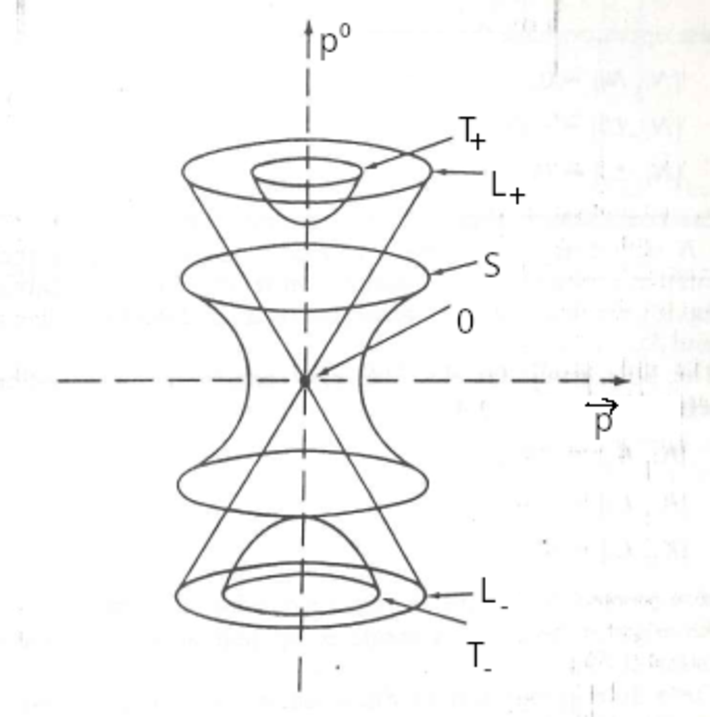
\includegraphics[width=0.7\textwidth]{pics/orbits}
    \caption{Kategorije mogućih orbita vektora u prostoru Minkowskog.}
    \label{fig:orbite}
\end{figure}
a pogodni reprezentanti i pripadajuće male grupe su
\begin{center}
\renewcommand{\arraystretch}{1.3}
\begin{tabular}{cccc}
\hline
\multicolumn{2}{c}{orbita} & reprezentant $p^*$ & mala grupa \\ \hline
    T$_+$ & $p^2=m^2>0$, $p^0>0$ &  $(m, 0, 0, 0)$  &  \SO{3} \\
    T$_-$ & $p^2=m^2>0$, $p^0<0$ &  $(-m, 0, 0, 0)$  &  \SO{3} \\
    L$_+$ & $p^2=0, p^0>0$ &  $(\omega, 0, 0, \omega)$  &  \ISO{2} \\
    L$_-$ & $p^2=0, p^0<0$ &  $(-\omega, 0, 0, \omega)$  &  \ISO{2} \\
    S & $p^2= - \kappa^2 < 0$ &  $(0, 0, 0, \kappa)$  &  \SO{1,2} \\
    0 & $p^{\mu} =  0$ &  $(0, 0, 0, 0)$  &  Poincar\'{e} \\
\end{tabular}
\renewcommand{\arraystretch}{1.0}
\end{center}
Za ovu kategorizaciju je prvenstveno iskorištena činjenica da je
kvadrat četverovektora $p^2$ invarijanta, što općenito dijeli četverovektore
na one vremenskog tipa (T), $p^2>0$, svjetlosnog tipa (L), $p^2=0$ i prostornog tipa (S),
$p^2<0$.
Nadalje, za  $p^2 \ge 0$ i predznak od $p^0$ je invarijantan (uvjerite se u to),
što cijepa kategorije T i L na dvije podkategorije.
Stanja iz kategorija T$_-$, L$_-$ i S nisu dosad identificirana u prirodi pa ih
nećemo razmatrati.
Kategorija 0 predstavlja vakuum koji je invarijantan na cijelu Poincar\'{e}ovu
grupu pa je odgovarajuća reprezentacija trivijalna i ne trebamo je
dalje razmatrati.
Kategoriju T$_+$ smo upravo razmotrili gore.
Tako nam preostaje razmotriti kategoriju L$_+$ bezmasenih stanja pozitivne
energije kojoj pripadaju npr. fotoni.

Fotoni nemaju sustav mirovanja pa je najjednostavniji reprezentant
oblika $k^{*\mu} = (\omega, 0, 0, \omega)$. Očito je da ovaj put
mala grupa \emph{nije} grupa rotacija. Jedino rotacije oko $z$-osi
$\{R(\theta) \td \theta \in [0, 2\pi)\}$ ostavljaju $k^{*\mu}$
invarijantan. Malu grupu kompletiraju dvoparametarske translacije
u $t-z$ "ravnini" dane matricom
\begin{equation}
  T(\vec{u}) = \begin{pmatrix}
      1+\vec{u}^2/2 & u_1 & u_2 & -\vec{u}^2/2 \\
u_1 & 1 & 0 & -u_1 \\
u_2 & 0 & 1 & -u_2 \\
\vec{u}/2 & u_1 & u_2 & 1-\vec{u}^2/2
  \end{pmatrix} \,,
    \label{eq:defTu}
\end{equation}
parametriziranom vektorom $\vec{u} = (u_1, u_2) \in \mathbb{R}^2$.
Čitatelj će se lako eksplicitnim množenjem uvjeriti da vrijedi
\begin{equation}
    \tensor{T(\vec{u})}{^{\mu}_{\nu}} k^{*\nu} = k^{*\mu} \,,
\end{equation}
a također i
\begin{align}
    T(\vec{u}) T(\vec{v}) &= T(\vec{u} + \vec{v}) \,, \\
    R(\theta) T(\vec{u}) R(\theta)^{-1} &= T(R(\theta)\vec{u}) \,,
\end{align}
uz $R(\theta)\vec{u} = (u_1\cos\theta + u_2 \sin\theta, -u_1\sin\theta+u_2\cos\theta)$,
što potvrđuje interpretaciju $T$ kao translacije i pokazuje da je mala grupa
od $k^{*}$ troparametarska grupa translacija i rotacija 2D prostora poznata
kao \emph{euklidska} grupa \ISO{2}, kako je i naznačeno u gornjoj tablici.
Baza odgovarajućeg malog Hilbertovog prostora $\mathcal{H}_{k^*}$ bit
će razapeta vektorima
\begin{equation}
  \ket{\vec{k}^{*}, \sigma} = \ket{\vec{k}^{*}, t_1, t_{2}, \lambda} \,,
\end{equation}
gdje je $\lambda$ svojstvena vrijednost od $J_z$ koju ćemo po analogiji
s masivnim slučajem zvati helicitet, a $t_{1,2}\in\mathbb{R}$,
su svojstvene
vrijednosti infinitezimalnih generatora translacija $T$ (odredite ih, vidi
zadatak \ref{zad:iso2gen}).
Jedino izolirano jednočestično bezmaseno stanje koje smo dosad opazili
u prirodi je foton koji u eksperimentima ne pokazuje nikakve značajke
koje bi ukazivale na posjedovanje dodatnog kontinuiranog kvantnog broja
$t_i$ pa smo prisiljeni zaključiti da je za foton $t_1=t_2=0$,
te da priroda nije iskoristila mogućnost $t_i \neq 0$.
Stavimo onda $t_1=t_2=0$ i promotrimo mali Hilbertov prostor
razapet s $\ket{\vec{k}^{*}, \lambda} \equiv \ket{\vec{k}^{*}, 0, 0, \lambda}$.
Kako mala grupa ne sadrži
operatore dizanja i spuštanja $J_{\pm}$, njenim djelovanjem $\lambda$
se ne mijenja\footnote{Operatori translacije isto ne mijenjaju $\lambda$
    za stanja s $t_1=t_2=0$ u što se lako možete uvjeriti nakon što
ste odredili komutacijske relacije u zadatku \ref{zad:iso2gen}.
Ispostavlja se da je ta translacijska simetrija povezana s tzv.
baždarnom simetrijom kvantne elektrodinamike, vidi \cite{Weinberg:1995mt}.}
i posljedično je mali Hilbertov prostor \emph{jednodimenzionalan} i
ponašanje bezmasenih stanja pri
transformacijama iz Poincar\'{e}ove grupe 
$(\Lambda, a) \in \mathbb{R}^{1,3}\rtimes\SOsup{+}{1,3}$ je jednostavno
\begin{equation}
    U(\Lambda, a) \ket{\vec{k}, \lambda} = e^{\rmi k\cdot a}
    e^{-\rmi \lambda \theta(\Lambda, k)} \ket{\Lambda\vec{k}, \lambda} \,,
    \label{eq:Urepm0}
\end{equation}
gdje je kut $\theta(\Lambda, k)$ potrebno odrediti netrivijalnim postupkom slično kao
i Wignerovu rotaciju u masivnom slučaju.
Uočite da stanja sa suprotnim helicitetima $\lambda$ i $-\lambda$ pripadaju
različitim reprezentacijama
i s tog stanovišta su lijevi i desni foton dvije različite čestice.
No ako proširimo grupu i s operatorom prostorne inverzije $P\in \O{1,3}$, slično kao za Diracovu
reprezentaciju u odjeljku \ref{sec:genLor}, ustanovili bi da
on mijenja predznak od $\lambda$ pa je u kontekstu teorija koje
imaju simetriju na prostornu inverziju, a takav je elektromagnetizam,
ipak prirodno desni ($\lambda=1$) i lijevi ($\lambda=-1)$ 
foton smatrati dvama stanjima iste čestice.

Zadnja finesa je da ništa dosad rečeno ne ograničava helicitet $\lambda$
da ne bude bilo koji realni broj. Sjetimo se naime da je kvantizacija
spina u \ref{ch:rotacije}. poglavlju bila posljedica \soAlg{3} algebre
koju ovdje nemamo. Međutim, ovisnost o $\lambda$
u (\ref{eq:Urepm0}) je samo kroz fazu, a kako je Poincar\'{e}ova grupa
dvostruko povezana (nasljeđeno od njene \SO{3} podgrupe rotacija),
rotacije za $\theta=2\pi$ smiju rezultirati samo fazom $\pm 1$ i
slijedi da je ipak $\lambda \in \{0, \fhalf, 1, \ldots\}$. Razlog
da je spin bezmasenih čestica polucjelobrojan nije posljedica
algebre (okoline jediničnog elementa) nego topologije (globalne strukture)
grupe simetrija.





\subsection*{Zadaci}

\begin{enumerate}[label=\arabic{chapter}.\arabic*.]

\item Uvjerite se eksplicitno da (\ref{eq:4DLorKom}) sadrži npr. (\ref{eq:LK3}).

\item Uvjerite se eksplicitno da (\ref{eq:4DJmn}) daje npr. (\ref{eq:defKi}).

\item Uvjerite se da generatori $J^{\mu\nu}$ definirani putem
(\ref{eq:DiracJ}) i (\ref{eq:DiracGamma}) zadovoljavaju komutacijske
relacije Lorentzove grupe (\ref{eq:4DLorKom}).

\item Uočite da je u trodimenzionalnom euklidskom prostoru pod djelovanjem grupe rotacija \SO{3}
    orbita vektora $\hat{\vec{z}} = (0, 0, 1)$ sfera $S^2$, a da je odgovarajuća
    mala grupa \SO{2}. Zatim konstruirajte bijekciju između te sfere i kvocijentnog
    skupa \SO{3}/\SO{2}. Općenito postojanje takve bijekcije tj. činjenica da je
    kvocijentni skup po maloj grupi (stabilizatoru)
    jednak orbiti poznato je kao \emph{teorem orbite i stabilizatora}.

\item Pokažite da helicitet $\vec{J}\cdot\vec{\hat{p}}$ komutira s impulsom $\vec{P}$.
    \label{zad:help}

\item Odredite inifinitezimalne generatore dvodimenzionalne euklidske
    grupe $\ISO{2}$ i njihove komutacijske relacije.\label{zad:iso2gen}
\end{enumerate}
